\chapter{Set up development environment} \label{appendix:devsetup}
Include how to setup the development environment for continuing developing on the library
\newpage
\chapter{Using Evothings in development process} \label{appendix:evothings}
Include how to troubleshoot and test with evothings
\newpage
\chapter{Deploying Evothings applications}
Comments on how to go from evothings applications to apps deployed or downloadable apks.
\newpage

\chapter{Provided examples} \label{appendix:examples}
Describe the different examples with screenshots and descriptions
\newpage
\chapter{Implemented tokens} \label{appendix:tokens}
\section{AnyBoard Token} \label{appendix:anyboard_token}
\subsection{Driver}
Describe the drivers
\subsection{Firmware}
Describe the firmware

\newpage
\section{AnyBoard Bean} \label{appendix:anyboard_bean}
\subsection{Driver}
Describe the drivers
\subsection{Firmware}
Describe the firmware
\newpage
\section{AnyBoard Bean Printer} \label{appendix:anyboard_bean_printer}
\subsection{Driver}
Describe the drivers
\subsection{Firmware}
Describe the firmware
\newpage
\chapter{AnyBoard Tests} \label{appendix:tests}

Desribe the tests.

\newpage
\chapter{BlueTooth communication protocol}
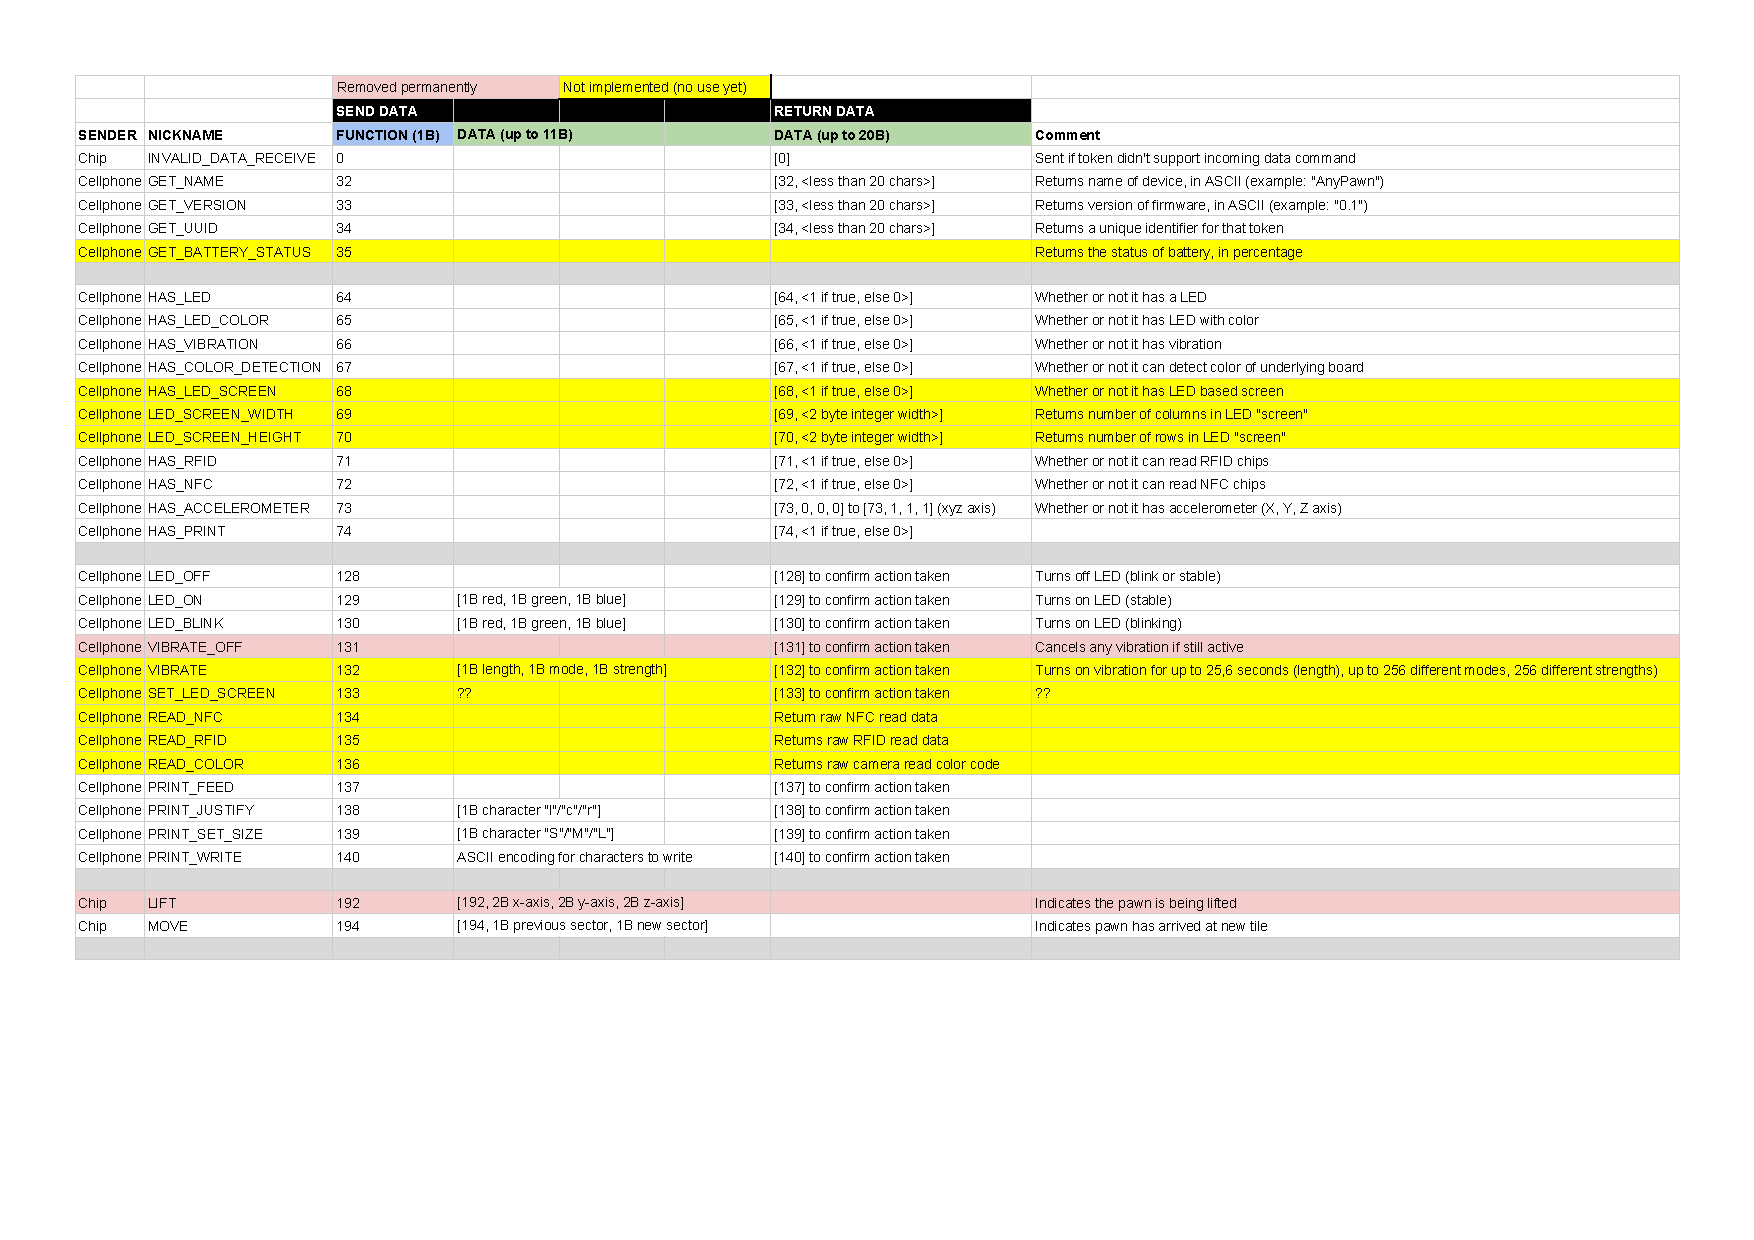
\includepdf[pages=-]{appendix/bluetooth_protocol.pdf}

\chapter{Article: Reflections on AnyBoard} \label{appendix:article}

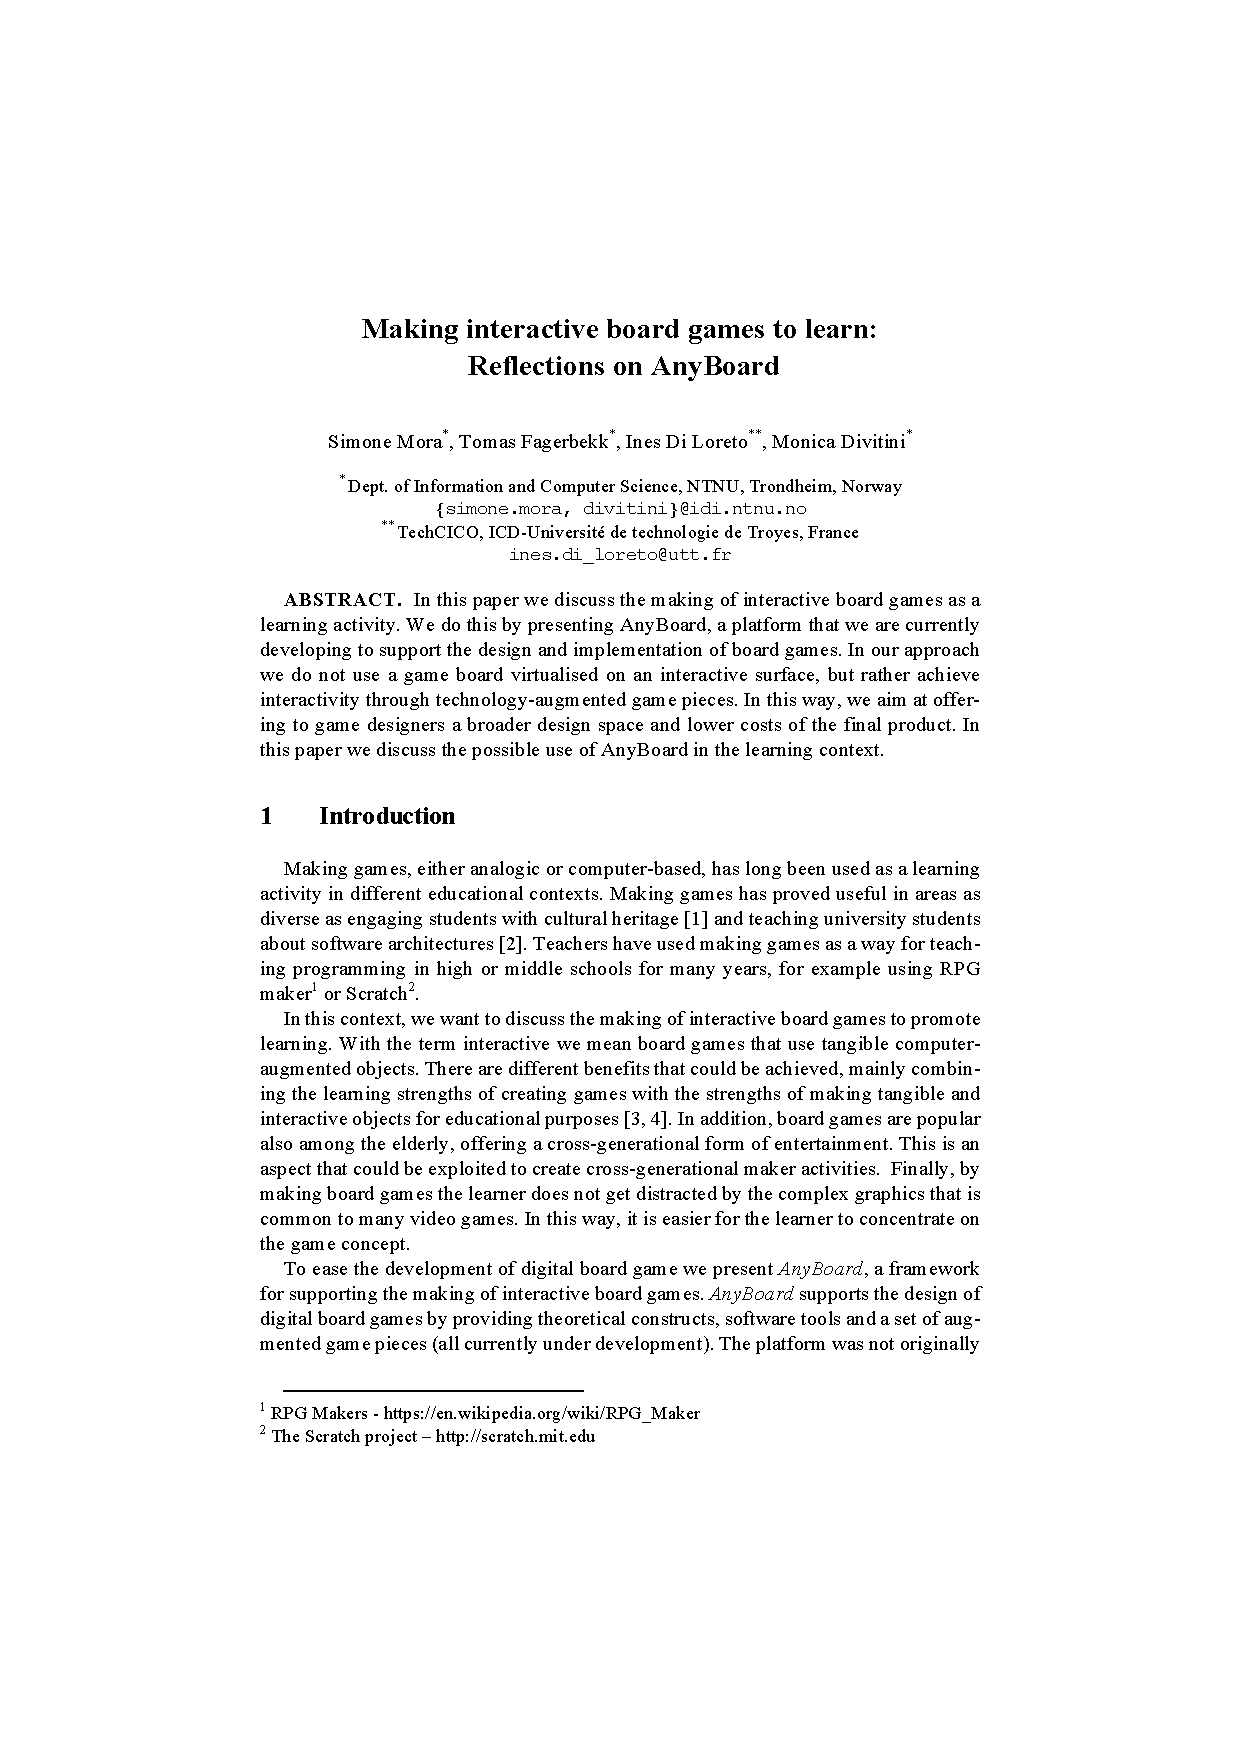
\includepdf[pages=-]{appendix/reflections_anyboard.pdf}

\chapter{AnyBoard Documentation} \label{appendix:doc}

Below is the complete documentation of the AnyBoard library pr. September 2015. This excludes drivers, which is not considered a part of the library. The documentation is also available in interactive format at \href{https://github.com/tomfa/anyboardjs/}{github.com/tomfa/anyboardjs}.

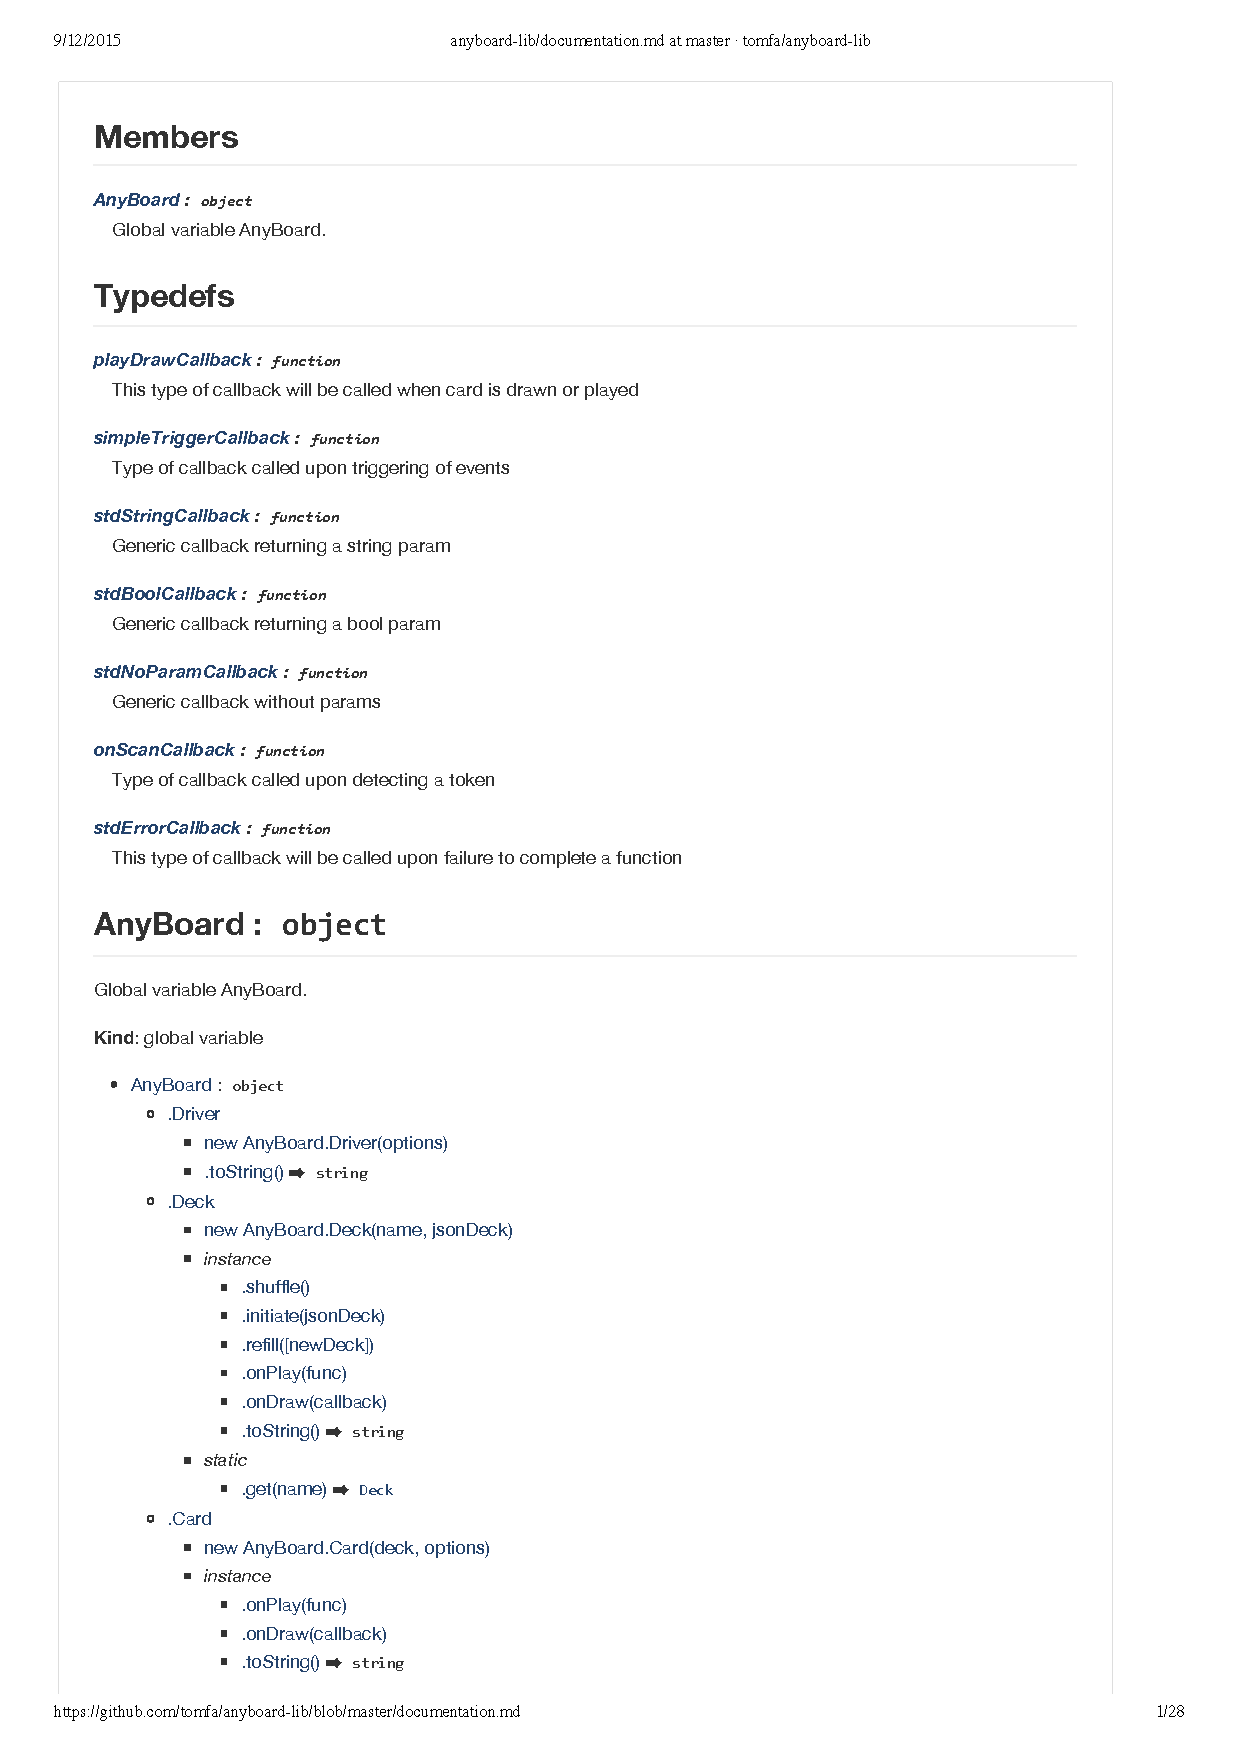
\includepdf[pages=-]{appendix/anyboard-lib_documentation.pdf}
\newpage
